\documentclass{minimal}
\usepackage[a4paper,margin=1cm,landscape]{geometry}
\usepackage{tikz}
\usetikzlibrary{positioning,shadows,arrows}

\begin{document}
\begin{center}
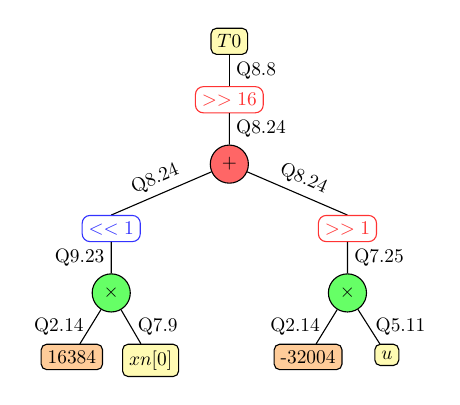
\begin{tikzpicture}[
     dec1/.style={rectangle, draw=red!80, rounded corners=1mm, fill=white,
        text centered, anchor=north, text=red!80, scale = 0.7},
    dec2/.style={rectangle, draw=blue!80, rounded corners=1mm, fill=white,
        text centered, anchor=north, text=blue!80, scale = 0.7},
    adder/.style={circle, draw, fill=red!60,
        text centered, anchor=north, text=black, scale = 0.7},
    mult/.style={circle, draw, fill=green!60,
        text centered, anchor=north, text=black, scale = 0.7},
     cst/.style={rectangle, rounded corners=0.7mm, draw, fill=orange!40,
        text centered, anchor=north, text=black, scale = 0.7},
     var/.style={rectangle, rounded corners=0.7mm, draw, fill=yellow!30,
        text centered, anchor=north, text=black, scale = 0.7},
     fpr/.style = {scale = 0.7},
    level distance=0.4cm, growth parent anchor=south
]
\node (Sortie) [var] {$T0$}
child{[sibling distance=3.000000cm]
	node(DAdd_0) [dec1] {$>>16 $}
	child{
		node(Add_0) [adder] {$+$}
	child{[sibling distance=1cm]
		node(DMultxn0 gamma  23) [dec2] {$<<1 $}
		child{
			node(Multxn0 gamma  23) [mult] {$\times$}
			child{
				node(Cst0) [cst] {16384}
			edge from parent node[fpr, left] {Q2.14}
			}
			child{
				node(Var0) [var] {$xn[0]$}
			edge from parent node[fpr, right] {Q7.9}
			}
			edge from parent node[fpr, left] {Q9.23}
		}
		edge from parent node[fpr, left,sloped,above] {Q8.24}
	}
	child{[sibling distance=1cm]
		node(DMultu gamma  25) [dec1] {$>>1 $}
		child{
			node(Multu gamma  25) [mult] {$\times$}
			child{
				node(Cst1) [cst] {-32004}
			edge from parent node[fpr, left] {Q2.14}
			}
			child{
				node(Var1) [var] {$u$}
			edge from parent node[fpr, right] {Q5.11}
			}
			edge from parent node[fpr, right] {Q7.25}
		}
		edge from parent node[fpr, right,sloped,above] {Q8.24}
	}
		edge from parent node[fpr, right] {Q8.24}	}
	edge from parent node[fpr, right] {Q8.8}
}

;

        
\end{tikzpicture}
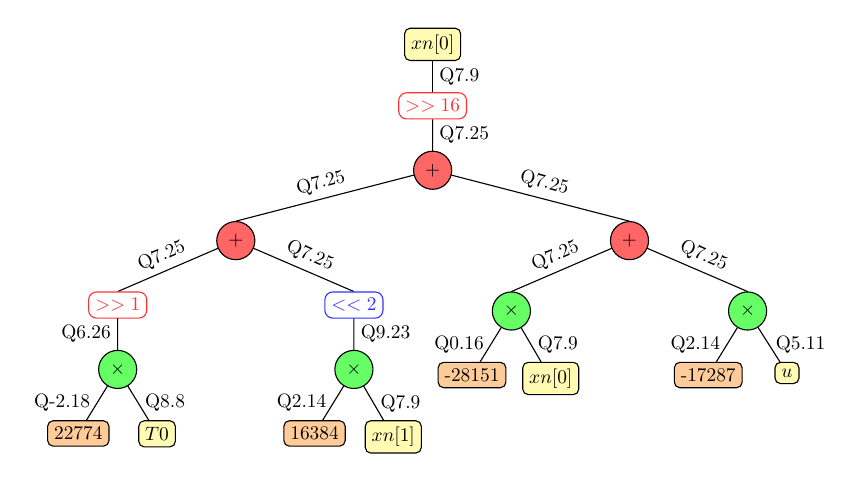
\begin{tikzpicture}[
     dec1/.style={rectangle, draw=red!80, rounded corners=1mm, fill=white,
        text centered, anchor=north, text=red!80, scale = 0.7},
    dec2/.style={rectangle, draw=blue!80, rounded corners=1mm, fill=white,
        text centered, anchor=north, text=blue!80, scale = 0.7},
    adder/.style={circle, draw, fill=red!60,
        text centered, anchor=north, text=black, scale = 0.7},
    mult/.style={circle, draw, fill=green!60,
        text centered, anchor=north, text=black, scale = 0.7},
     cst/.style={rectangle, rounded corners=0.7mm, draw, fill=orange!40,
        text centered, anchor=north, text=black, scale = 0.7},
     var/.style={rectangle, rounded corners=0.7mm, draw, fill=yellow!30,
        text centered, anchor=north, text=black, scale = 0.7},
     fpr/.style = {scale = 0.7},
    level distance=0.4cm, growth parent anchor=south
]
\node (Sortie) [var] {$xn[0]$}
child{[sibling distance=5.000000cm]
	node(DAdd_34) [dec1] {$>>16 $}
	child{
		node(Add_34) [adder] {$+$}
	child{[sibling distance=3.000000cm]
		node(Add_33) [adder] {$+$}
		child{[sibling distance=1cm]
			node(DMultT0 gamma  26) [dec1] {$>>1 $}
			child{
				node(MultT0 gamma  26) [mult] {$\times$}
				child{
					node(Cst2) [cst] {22774}
				edge from parent node[fpr, left] {Q-2.18}
				}
				child{
					node(Var2) [var] {$T0$}
				edge from parent node[fpr, right] {Q8.8}
				}
				edge from parent node[fpr, left] {Q6.26}
			}
			edge from parent node[fpr, left,sloped,above] {Q7.25}
		}
		child{[sibling distance=1cm]
			node(DMultxn1 gamma  23) [dec2] {$<<2 $}
			child{
				node(Multxn1 gamma  23) [mult] {$\times$}
				child{
					node(Cst3) [cst] {16384}
				edge from parent node[fpr, left] {Q2.14}
				}
				child{
					node(Var3) [var] {$xn[1]$}
				edge from parent node[fpr, right] {Q7.9}
				}
				edge from parent node[fpr, right] {Q9.23}
			}
			edge from parent node[fpr, right,sloped,above] {Q7.25}
		}
		edge from parent node[fpr, left,sloped,above] {Q7.25}
	}
	child{[sibling distance=3.000000cm]
		node(Add_1) [adder] {$+$}
		child{[sibling distance=1cm]
			node(Multxn0 gamma  25) [mult] {$\times$}
			child{
				node(Cst0) [cst] {-28151}
			edge from parent node[fpr, left] {Q0.16}
			}
			child{
				node(Var0) [var] {$xn[0]$}
			edge from parent node[fpr, right] {Q7.9}
			}
			edge from parent node[fpr, left,sloped,above] {Q7.25}
		}
		child{[sibling distance=1cm]
			node(Multu gamma  25) [mult] {$\times$}
			child{
				node(Cst1) [cst] {-17287}
			edge from parent node[fpr, left] {Q2.14}
			}
			child{
				node(Var1) [var] {$u$}
			edge from parent node[fpr, right] {Q5.11}
			}
			edge from parent node[fpr, right,sloped,above] {Q7.25}
		}
		edge from parent node[fpr, right,sloped,above] {Q7.25}
	}
		edge from parent node[fpr, right] {Q7.25}	}
	edge from parent node[fpr, right] {Q7.9}
}

;
        
\end{tikzpicture}
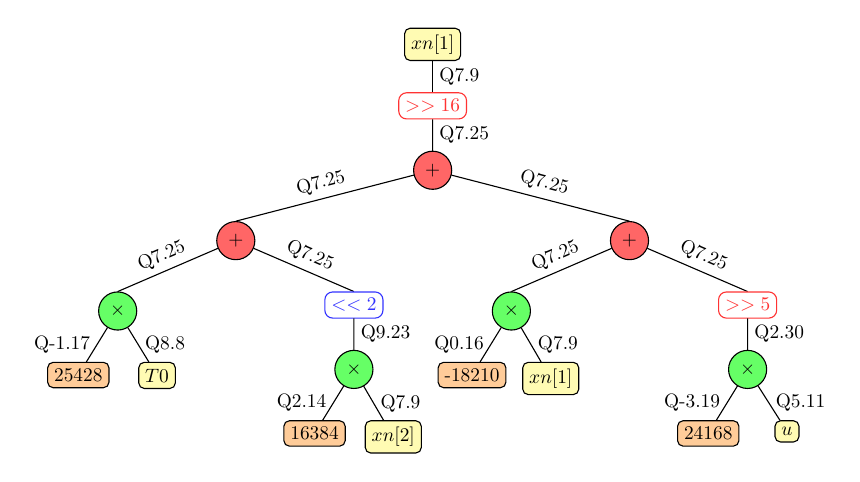
\begin{tikzpicture}[
     dec1/.style={rectangle, draw=red!80, rounded corners=1mm, fill=white,
        text centered, anchor=north, text=red!80, scale = 0.7},
    dec2/.style={rectangle, draw=blue!80, rounded corners=1mm, fill=white,
        text centered, anchor=north, text=blue!80, scale = 0.7},
    adder/.style={circle, draw, fill=red!60,
        text centered, anchor=north, text=black, scale = 0.7},
    mult/.style={circle, draw, fill=green!60,
        text centered, anchor=north, text=black, scale = 0.7},
     cst/.style={rectangle, rounded corners=0.7mm, draw, fill=orange!40,
        text centered, anchor=north, text=black, scale = 0.7},
     var/.style={rectangle, rounded corners=0.7mm, draw, fill=yellow!30,
        text centered, anchor=north, text=black, scale = 0.7},
     fpr/.style = {scale = 0.7},
    level distance=0.4cm, growth parent anchor=south
]
\node (Sortie) [var] {$xn[1]$}
child{[sibling distance=5.000000cm]
	node(DAdd_63) [dec1] {$>>16 $}
	child{
		node(Add_63) [adder] {$+$}
	child{[sibling distance=3.000000cm]
		node(Add_62) [adder] {$+$}
		child{[sibling distance=1cm]
			node(MultT0 gamma  25) [mult] {$\times$}
			child{
				node(Cst2) [cst] {25428}
			edge from parent node[fpr, left] {Q-1.17}
			}
			child{
				node(Var2) [var] {$T0$}
			edge from parent node[fpr, right] {Q8.8}
			}
			edge from parent node[fpr, left,sloped,above] {Q7.25}
		}
		child{[sibling distance=1cm]
			node(DMultxn2 gamma  23) [dec2] {$<<2 $}
			child{
				node(Multxn2 gamma  23) [mult] {$\times$}
				child{
					node(Cst3) [cst] {16384}
				edge from parent node[fpr, left] {Q2.14}
				}
				child{
					node(Var3) [var] {$xn[2]$}
				edge from parent node[fpr, right] {Q7.9}
				}
				edge from parent node[fpr, right] {Q9.23}
			}
			edge from parent node[fpr, right,sloped,above] {Q7.25}
		}
		edge from parent node[fpr, left,sloped,above] {Q7.25}
	}
	child{[sibling distance=3.000000cm]
		node(Add_37) [adder] {$+$}
		child{[sibling distance=1cm]
			node(Multxn1 gamma  25) [mult] {$\times$}
			child{
				node(Cst0) [cst] {-18210}
			edge from parent node[fpr, left] {Q0.16}
			}
			child{
				node(Var0) [var] {$xn[1]$}
			edge from parent node[fpr, right] {Q7.9}
			}
			edge from parent node[fpr, left,sloped,above] {Q7.25}
		}
		child{[sibling distance=1cm]
			node(DMultu gamma  30) [dec1] {$>>5 $}
			child{
				node(Multu gamma  30) [mult] {$\times$}
				child{
					node(Cst1) [cst] {24168}
				edge from parent node[fpr, left] {Q-3.19}
				}
				child{
					node(Var1) [var] {$u$}
				edge from parent node[fpr, right] {Q5.11}
				}
				edge from parent node[fpr, right] {Q2.30}
			}
			edge from parent node[fpr, right,sloped,above] {Q7.25}
		}
		edge from parent node[fpr, right,sloped,above] {Q7.25}
	}
		edge from parent node[fpr, right] {Q7.25}	}
	edge from parent node[fpr, right] {Q7.9}
}

;
        
\end{tikzpicture}

\hspace{3cm}

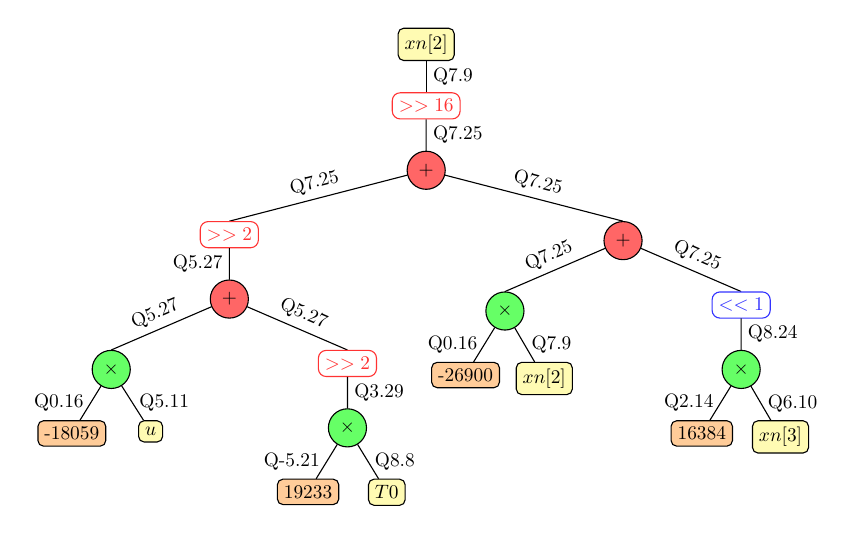
\begin{tikzpicture}[
     dec1/.style={rectangle, draw=red!80, rounded corners=1mm, fill=white,
        text centered, anchor=north, text=red!80, scale = 0.7},
    dec2/.style={rectangle, draw=blue!80, rounded corners=1mm, fill=white,
        text centered, anchor=north, text=blue!80, scale = 0.7},
    adder/.style={circle, draw, fill=red!60,
        text centered, anchor=north, text=black, scale = 0.7},
    mult/.style={circle, draw, fill=green!60,
        text centered, anchor=north, text=black, scale = 0.7},
     cst/.style={rectangle, rounded corners=0.7mm, draw, fill=orange!40,
        text centered, anchor=north, text=black, scale = 0.7},
     var/.style={rectangle, rounded corners=0.7mm, draw, fill=yellow!30,
        text centered, anchor=north, text=black, scale = 0.7},
     fpr/.style = {scale = 0.7},
    level distance=0.4cm, growth parent anchor=south
]
\node (Sortie) [var] {$xn[2]$}
child{[sibling distance=5.000000cm]
	node(DAdd_83) [dec1] {$>>16 $}
	child{
		node(Add_83) [adder] {$+$}
	child{[sibling distance=3.000000cm]
		node(DAdd_82) [dec1] {$>>2 $}
		child{
			node(Add_82) [adder] {$+$}
		child{[sibling distance=1cm]
			node(Multu gamma  27) [mult] {$\times$}
			child{
				node(Cst1) [cst] {-18059}
			edge from parent node[fpr, left] {Q0.16}
			}
			child{
				node(Var1) [var] {$u$}
			edge from parent node[fpr, right] {Q5.11}
			}
			edge from parent node[fpr, left,sloped,above] {Q5.27}
		}
		child{[sibling distance=1cm]
			node(DMultT0 gamma  29) [dec1] {$>>2 $}
			child{
				node(MultT0 gamma  29) [mult] {$\times$}
				child{
					node(Cst2) [cst] {19233}
				edge from parent node[fpr, left] {Q-5.21}
				}
				child{
					node(Var2) [var] {$T0$}
				edge from parent node[fpr, right] {Q8.8}
				}
				edge from parent node[fpr, right] {Q3.29}
			}
			edge from parent node[fpr, right,sloped,above] {Q5.27}
		}
			edge from parent node[fpr, left] {Q5.27}		}
		edge from parent node[fpr, left,sloped,above] {Q7.25}
	}
	child{[sibling distance=3.000000cm]
		node(Add_69) [adder] {$+$}
		child{[sibling distance=1cm]
			node(Multxn2 gamma  25) [mult] {$\times$}
			child{
				node(Cst0) [cst] {-26900}
			edge from parent node[fpr, left] {Q0.16}
			}
			child{
				node(Var0) [var] {$xn[2]$}
			edge from parent node[fpr, right] {Q7.9}
			}
			edge from parent node[fpr, left,sloped,above] {Q7.25}
		}
		child{[sibling distance=1cm]
			node(DMultxn3 gamma  24) [dec2] {$<<1 $}
			child{
				node(Multxn3 gamma  24) [mult] {$\times$}
				child{
					node(Cst3) [cst] {16384}
				edge from parent node[fpr, left] {Q2.14}
				}
				child{
					node(Var3) [var] {$xn[3]$}
				edge from parent node[fpr, right] {Q6.10}
				}
				edge from parent node[fpr, right] {Q8.24}
			}
			edge from parent node[fpr, right,sloped,above] {Q7.25}
		}
		edge from parent node[fpr, right,sloped,above] {Q7.25}
	}
		edge from parent node[fpr, right] {Q7.25}	}
	edge from parent node[fpr, right] {Q7.9}
}

;
        
\end{tikzpicture}
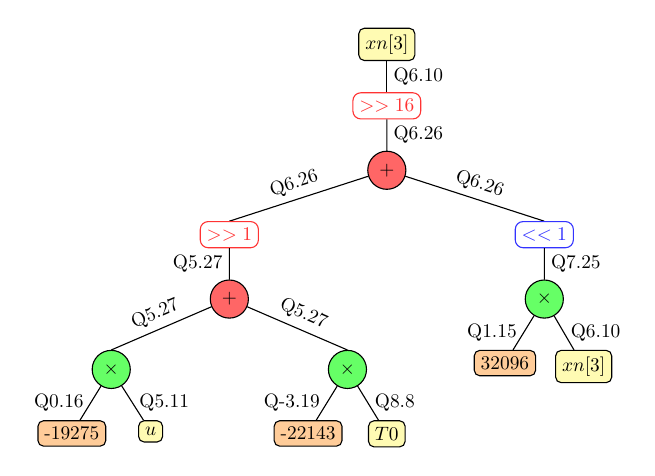
\begin{tikzpicture}[
     dec1/.style={rectangle, draw=red!80, rounded corners=1mm, fill=white,
        text centered, anchor=north, text=red!80, scale = 0.7},
    dec2/.style={rectangle, draw=blue!80, rounded corners=1mm, fill=white,
        text centered, anchor=north, text=blue!80, scale = 0.7},
    adder/.style={circle, draw, fill=red!60,
        text centered, anchor=north, text=black, scale = 0.7},
    mult/.style={circle, draw, fill=green!60,
        text centered, anchor=north, text=black, scale = 0.7},
     cst/.style={rectangle, rounded corners=0.7mm, draw, fill=orange!40,
        text centered, anchor=north, text=black, scale = 0.7},
     var/.style={rectangle, rounded corners=0.7mm, draw, fill=yellow!30,
        text centered, anchor=north, text=black, scale = 0.7},
     fpr/.style = {scale = 0.7},
    level distance=0.4cm, growth parent anchor=south
]
\node (Sortie) [var] {$xn[3]$}
child{[sibling distance=4.000000cm]
	node(DAdd_105) [dec1] {$>>16 $}
	child{
		node(Add_105) [adder] {$+$}
	child{[sibling distance=3.000000cm]
		node(DAdd_104) [dec1] {$>>1 $}
		child{
			node(Add_104) [adder] {$+$}
		child{[sibling distance=1cm]
			node(Multu gamma  27) [mult] {$\times$}
			child{
				node(Cst1) [cst] {-19275}
			edge from parent node[fpr, left] {Q0.16}
			}
			child{
				node(Var1) [var] {$u$}
			edge from parent node[fpr, right] {Q5.11}
			}
			edge from parent node[fpr, left,sloped,above] {Q5.27}
		}
		child{[sibling distance=1cm]
			node(MultT0 gamma  27) [mult] {$\times$}
			child{
				node(Cst2) [cst] {-22143}
			edge from parent node[fpr, left] {Q-3.19}
			}
			child{
				node(Var2) [var] {$T0$}
			edge from parent node[fpr, right] {Q8.8}
			}
			edge from parent node[fpr, right,sloped,above] {Q5.27}
		}
			edge from parent node[fpr, left] {Q5.27}		}
		edge from parent node[fpr, left,sloped,above] {Q6.26}
	}
	child{[sibling distance=1cm]
		node(DMultxn3 gamma  25) [dec2] {$<<1 $}
		child{
			node(Multxn3 gamma  25) [mult] {$\times$}
			child{
				node(Cst0) [cst] {32096}
			edge from parent node[fpr, left] {Q1.15}
			}
			child{
				node(Var0) [var] {$xn[3]$}
			edge from parent node[fpr, right] {Q6.10}
			}
			edge from parent node[fpr, right] {Q7.25}
		}
		edge from parent node[fpr, right,sloped,above] {Q6.26}
	}
		edge from parent node[fpr, right] {Q6.26}	}
	edge from parent node[fpr, right] {Q6.10}
}

;
        
\end{tikzpicture}

\end{center}
\end{document}